\section{Project Organization and Programming Notes}

\subsection{Overview}
\begin{itemize}
    \item The project is divided into several components with distinct functions.
    \item The structure of the program is strictly built by a range of folders and files. Particularly, the projects comprises algorithm implementations, test cases, other functions to operate the program. Those components are linked by header files.
\end{itemize}

\subsection{Main Functions}
\begin{itemize}
    \item Sorting Algorithm Implementations
    \begin{itemize}
        \item Selection Sort
        \item Insertion Sort
        \item Binary Insertion Sort
        \item Bubble Sort
        \item Heap Sort
        \item Merge Sort
        \item Quick Sort
        \item Shell Sort
        \item Flash Sort
        \item Radix Sort
        \item Counting Sort
        \item Shaker Sort
    \end{itemize}
    \item Data Generation
    \begin{itemize}
        \item Explanation
        \begin{itemize}
            \item Creating datasets uses for input of programming or making an input file based on four types: sorted, nearly sorted, reversed and randomized and six sizes such as 10000, 30000, $\ldots$ 500000.
            \item Tranversing datas from programming to output file when it is needed.
        \end{itemize}
        \item Pseudo code
        \begin{verbatim}
            1.  FUNCTION GenerateData(n, type)
            2.       create array A
            3.
            4.       if type == "-sorted"
            5.            for i = 0 to n-1: A[i] = i
            6.
            7.       else if type == "-rev"
            8.            for i = 0 to n-1: A[i] = n-1-i
            9.
            10.      else if type == "-rand"
            11.           set random seed
            12.           for i = 0 to n-1: A[i] = random(0, n-1)
            13.
            14.      else if type == "-nsorted"
            15.           for i = 0 to n-1: A[i] = i
            16.           repeat 10 times:
            17.                swap A[random(0,n-1)], A[random(0,n-1)]
            18.
            19.      return A
            20.
            21. FUNCTION WriteFile(n, type, filename)
            22.      open file
            23.      if fail → print error, stop
            24.
            25.      write n
            26.      A = GenerateData(n, type)
            27.
            28.      for each x in A: write x
            29.
            30.      close file
            31.
            32. FUNCTION WriteArray(filename, A)
            33.      open file
            34.      if success:
            35.           write size(A)
            36.           for i = 0 to size(A)-1:
            37.                write A[i]
            38.                if not last → write space
            39.           close file
            40.      else:
            41.           print error
        \end{verbatim}
    \end{itemize}
    \item Comparisons and Time Calculation
    \begin{itemize}
        \item Explanation
        \begin{itemize}
            \item Creating datasets uses for input of programming or making an input file based on four types: sorted, nearly sorted, reversed and randomized and six sizes such as 10000, 30000, $\ldots$ 500000.
            \item Tranversing datas from programming to output file when it is needed.
        \end{itemize}
        \item Pseudo code
        \begin{verbatim}
            1.  FUNCTION GetAlgorithm(name, A)
            2.       Tmp = copy of A
            3.       comparisons = 0
            4.       start = current time
            5.
            6.       if name == "selection-sort"
            7.            run selectionSortTime(Tmp)
            8.            end = current time
            9.            Tmp = copy of A
            10.           run selectionSort(Tmp, comparisons)
            11.
            12.      else if name == "insertion-sort"
            13.           run insertionSortTime(Tmp)
            14.           end = current time
            15.           Tmp = copy of A
            16.           run insertionSort(Tmp, comparisons)
            17.
            18.      ...
            19.      (repeat for other algorithms)
            20.
            21.      time = end - start
            22.      return (comparisons, time, Tmp)
            23.
            24. FUNCTION ReadFile(A, command)
            25.      open input file
            26.      if fail → print error, stop
            27.
            28.      read n
            29.      for i = 0 to n-1: read A[i]
            30.      close file
            31.
            32. FUNCTION MakeInput(A, command)
            33.      if "-rand" → A = GenerateData(n, "-rand")
            34.      if "-sorted" → A = GenerateData(n, "-sorted")
            35.      if "-rev" → A = GenerateData(n, "-rev")
            36.      if "-nsorted" → A = GenerateData(n, "-nsorted")
            37.
            38. FUNCTION Process(command)
            39.      if inputOrder == "-all" → return
            40.
            41.      declare A
            42.
            43.      if input file exists
            44.           ReadFile(A, command)
            45.      else
            46.           MakeInput(A, command)
            47.           write A to input file
            48.
            49.      (cmp1, time1, sorted1) = GetAlgorithm(algorithm1, A)
            50.
            51.      if mode == "-c"
            52.           (cmp2, time2, sorted2) = GetAlgorithm(algorithm2, A)
            53.
            54.      save results to command
            55.
            56.      if mode == "-a" and not command3
            57.           write sorted1 to output file
        \end{verbatim}
    \end{itemize}
    \item Command Processing
    \begin{itemize}
        \item Explanation
        \begin{itemize}
            \item Creating datasets uses for input of programming or making an input file based on four types: sorted, nearly sorted, reversed and randomized and six sizes such as 10000, 30000, $\ldots$ 500000.
            \item Tranversing datas from programming to output file when it is needed.
        \end{itemize}
        \item Pseudo code
        \begin{verbatim}
            1.  FUNCTION isNumber(s)
            2.       if s is empty → return false
            3.       for each character c in s
            4.            if c is not a digit → return false
            5.       return true
            6.
            7.  FUNCTION CommandProcessing(argc, argv)
            8.       create command
            9.
            10.      command.mode = argv[1]
            11.      command.algorithm1 = argv[2]
            12.
            13.      if command.mode == "-a"
            14.           if isNumber(argv[3])
            15.                command.inputSize = toInteger(argv[3])
            16.           else
            17.                command.inputFile = argv[3]
            18.
            19.           if argc == 5
            20.                command.outputParameter = argv[4]
            21.           else
            22.                command.inputOrder = argv[4]
            23.                command.outputParameter = argv[5]
            24.
            25.      else if command.mode == "-c"
            26.           command.algorithm2 = argv[3]
            27.
            28.           if isNumber(argv[4])
            29.                command.inputSize = toInteger(argv[4])
            30.                command.inputOrder = argv[5]
            31.           else
            32.                command.inputFile = argv[4]
            33.
            34.      return command
        \end{verbatim}
    \end{itemize}
    \item Console UI
    \begin{itemize}
        \item Explanation
        \begin{itemize}
            \item Output of programme, writting on consol
            \item Tranversing datas from programming to output file when it is needed.
        \end{itemize}
        \item Pseudo code
        \begin{verbatim}
            1.  FUNCTION OutputParameter(type, command)
            2.       if type == "-time"
            3.            print runningTime1
            4.            if algorithm2 exists → print " | " + runningTime2
            5.
            6.       else if type == "-comp"
            7.            print comparisons1
            8.            if algorithm2 exists → print " | " + comparisons2
            9.
            10.      else
            11.           print runningTime1 (+ runningTime2 if exists)
            12.           print comparisons1 (+ comparisons2 if exists)
            13.
            14. FUNCTION AlgorithmInputOrder(order)
            15.      if order == "-sorted" → return "Sorted"
            16.      if order == "-nsorted" → return "Nearly Sorted"
            17.      if order == "-rev" → return "Reverse Sorted"
            18.      if order == "-rand" → return "Randomized"
            19.      return ""
            20.
            21. FUNCTION NameAlgorithm(name)
            22.      map algorithm name string to readable name
            23.      (e.g., "quick-sort" → "Quick Sort")
            24.      return result
            25.
            26. FUNCTION ConsoleUI(command)
            27.      print algorithm1 (+ algorithm2 if exists)
            28.
            29.      if inputFile exists
            30.           print input file
            31.
            32.      print input size
            33.
            34.      if no input file
            35.           print input order
            36.
            37.      print separator line
            38.      call OutputParameter(command.outputParameter, command)
            39.
            40. FUNCTION Print(command)
            41.      if inputOrder == "-all" AND no input file
            42.           for each type in {"-sorted", "-nsorted", "-rev", "-rand"}
            43.                command.inputOrder = type
            44.                call getComparisonsAndTime(command)
            45.                call ConsoleUI(command)
            46.                print newline
            47.
            48.      else
            49.           call ConsoleUI(command)
        \end{verbatim}
    \end{itemize}
\end{itemize}

\subsection{File Organization}

\begin{itemize}

\item \textbf{Source}

\begin{itemize}

\item \textbf{sortAlgorithms}
\begin{itemize}
    \item \texttt{binaryInsertion.cpp}
    \item \texttt{bubbleSort.cpp}
    \item \texttt{countingSort.cpp}
    \item \texttt{flashSort.cpp}
    \item \texttt{heapSort.cpp}
    \item \texttt{insertionSort.cpp}
    \item \texttt{mergeSort.cpp}
    \item \texttt{quickSort.cpp}
    \item \texttt{radixSort.cpp}
    \item \texttt{selectionSort.cpp}
    \item \texttt{shakerSort.cpp}
    \item \texttt{shellSort.cpp}
    \item \texttt{sort.h}
\end{itemize}

\item \textbf{TestCases}
\begin{itemize}
    \item \texttt{sorted\_10000.txt}
    \item \texttt{sorted\_30000.txt}
    \item \texttt{sorted\_50000.txt}
    \item \texttt{sorted\_100000.txt}
    \item \texttt{sorted\_300000.txt}
    \item \texttt{sorted\_500000.txt}

    \item \texttt{nsorted\_10000.txt}
    \item \texttt{nsorted\_30000.txt}
    \item \texttt{nsorted\_50000.txt}
    \item \texttt{nsorted\_100000.txt}
    \item \texttt{nsorted\_300000.txt}
    \item \texttt{nsorted\_500000.txt}

    \item \texttt{rev\_10000.txt}
    \item \texttt{rev\_30000.txt}
    \item \texttt{rev\_50000.txt}
    \item \texttt{rev\_100000.txt}
    \item \texttt{rev\_300000.txt}
    \item \texttt{rev\_500000.txt}

    \item \texttt{rand\_10000.txt}
    \item \texttt{rand\_30000.txt}
    \item \texttt{rand\_50000.txt}
    \item \texttt{rand\_100000.txt}
    \item \texttt{rand\_300000.txt}
    \item \texttt{rand\_500000.txt}
\end{itemize}

\item \texttt{commandProcessing.cpp}
\item \texttt{commandProcessing.h}

\item \texttt{consoleUI.cpp}
\item \texttt{consoleUI.h}

\item \texttt{dataGeneration.cpp}
\item \texttt{dataGeneration.h}

\item \texttt{getComparisonsAndTime.cpp}
\item \texttt{getComparisonsAndTime.h}

\item \texttt{main.cpp}

\item \texttt{07.exe} (run file)

\end{itemize}

\end{itemize}
\newpage
\subsection{Program Running Process}
The execution of the program is demonstrated at the below chart.

\begin{figure}[h]
    \centering
    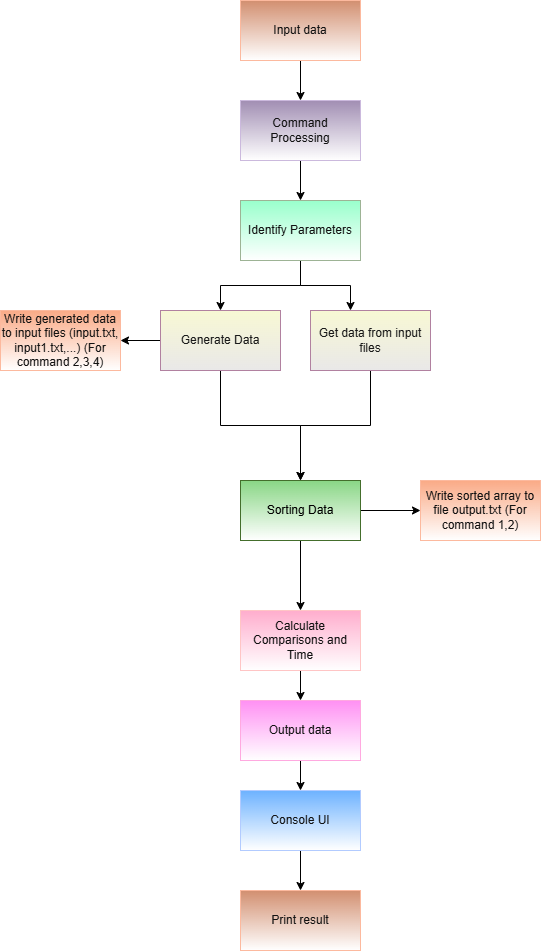
\includegraphics[width=0.6\linewidth]{img/programProcess.png}
    \caption{Program running process}
    \label{fig:process}
\end{figure}
